\begin{frame}[plain,noframenumbering]
    \centering
    \scalebox{3}{Understanding References}
\end{frame}

\section{Understanding References}

\begin{frame}[fragile]{Q: What is the output of the programs?}
    \begin{columns}[t]
        \begin{column}{.45\textwidth}
        \only<2>{A: \texttt{12}}

    \begin{lstlisting}[language=python]
#!/usr/bin/env python3

class S:
    def __init__(self, x):
        self.x = x

def swap(a, b):
    b, a = a, b

if __name__ == '__main__':
    a, b = S(1), S(2)
    swap(a, b)
    print(f'{a.x}{b.x}')
    \end{lstlisting}
        \end{column}
        \begin{column}{.45\textwidth}
            \only<2>{A: \texttt{22}}

            \inputcpplisting{snippet28a}
        \end{column}
    \end{columns}
\end{frame}

\begin{frame}[fragile]{Q: What is the output of the program?}
    \inputcpplisting{snippet28b}
\end{frame}

\begin{frame}[fragile]{A: \texttt{21}}
    \inputcpplisting{snippet28b}
\end{frame}

\begin{frame}[fragile]{Q: What is the output of the program?}
    \inputcpplisting{snippet28c}
\end{frame}

\begin{frame}[fragile]{A: \texttt{aacc22}}
    \inputcpplisting{snippet28c}
\end{frame}

\begin{frame}[fragile]{Q: What is the output of the program?}
    \inputcpplisting{snippet28d}
\end{frame}

\begin{frame}[fragile]{A: \texttt{aabcc21}}
    \inputcpplisting{snippet28d}
\end{frame}

\begin{frame}[fragile]{Q: What is the output of the program?}
    \inputcpplisting{snippet28e}
\end{frame}

\begin{frame}[fragile]{A: \texttt{aa12}}
    \inputcpplisting{snippet28e}
\end{frame}

\begin{frame}[fragile]{Q: What is the output of the program?}
    \inputcpplisting{snippet28f}
\end{frame}

\begin{frame}[fragile]{A: \texttt{aa12}}
    \inputcpplisting{snippet28f}
\end{frame}

\begin{frame}[fragile]{Q: What is the output of the program?}
    \inputcpplisting{snippet28g}
\end{frame}

\begin{frame}[fragile]{A: \texttt{aa21}}
    \inputcpplisting{snippet28g}
\end{frame}

\begin{frame}[fragile]{Q: What is the output of the program?}
    \only<2>{\textbf{\textcolor{vertexDarkRed}{error:}} cannot bind non-const lvalue reference of type \enquote{S*\&} to an rvalue of type \enquote{S*}}
    \inputcpplisting{snippet28h}
\end{frame}

\begin{frame}[plain,noframenumbering]
    \centering
    \scalebox{3}{Value Categories}
\end{frame}

\section{Value Categories}

\begin{frame}{Value categories with Venn diagrams}
    \centering

    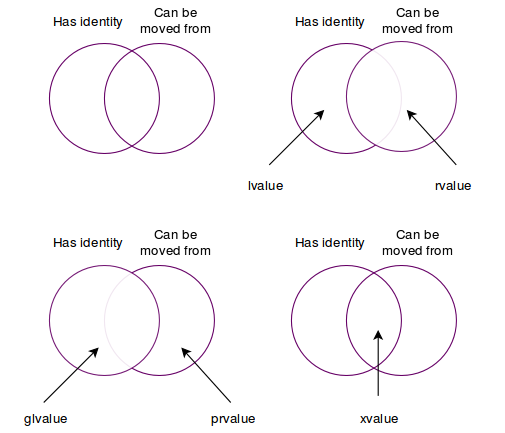
\includegraphics[height=.8\textheight]{valcat.png}

    \scalebox{.7}{(diagrams shamelessly stolen from \href{http://bajamircea.github.io/coding/cpp/2016/04/07/move-forward.html}{\texttt{bajamircea.github.io/coding/cpp/2016/04/07/move-forward.html}})}

\end{frame}

\begin{frame}[fragile]{Value categories with Venn diagrams}
    \begin{center}
        \scalebox{.7}{(diagrams shamelessly stolen from \href{http://bajamircea.github.io/coding/cpp/2016/04/07/move-forward.html}{\texttt{bajamircea.github.io/coding/cpp/2016/04/07/move-forward.html}})}
    \end{center}
    \begin{columns}
        \begin{column}{.7\textwidth}
            \begin{lstlisting}
struct S{ int x; };

S make_S(int x) {
    S s{.x = x};
    return s; // has no name after returning
}

int main() {
    S a = make_S(42); // `a` is an lvalue
                      // initialized with a prvalue

    S b = std::move(a); // prepare to die, `a`!
                        // now `a` became an xvalue

    auto x = a.x; // ERROR: `a` is in an undefined state
    a = make_S(13);
    x = a.x; // fine!
}
            \end{lstlisting}
        \end{column}
        \begin{column}{.25\textwidth}
            \only<1>{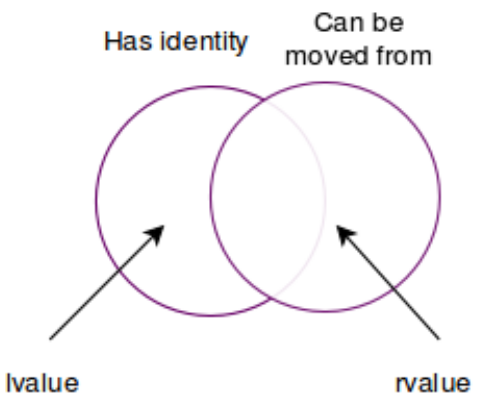
\includegraphics[width=\textwidth]{valcat1.png}}%
            \only<2>{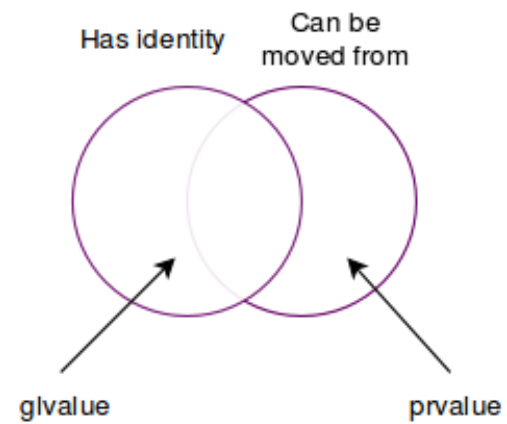
\includegraphics[width=\textwidth]{valcat2.png}}%
            \only<3>{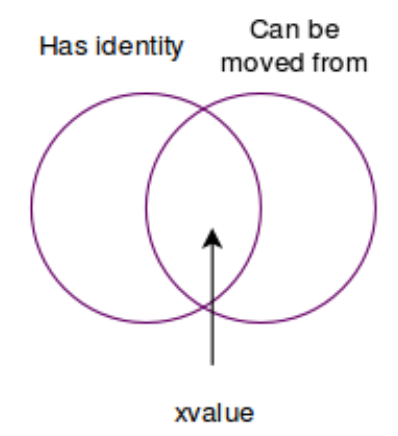
\includegraphics[width=\textwidth]{valcat3.png}}%
        \end{column}
    \end{columns}
\end{frame}

\begin{frame}[fragile]{Binding references to temporaries}
    \begin{center}
        \textbf{\textcolor{vertexDarkRed}{error:}} cannot bind non-const lvalue reference of type \enquote{S*\&} to an rvalue of type \enquote{S*}
    \end{center}
    \begin{columns}
        \begin{column}{.4\textwidth}
            \begin{lstlisting}
template <typename T>
void swap(T& a, T& b) { ... }

int main() {
    S a{1};
    S b{2};
    swap(&a, &b);
}
            \end{lstlisting}
        \end{column}
        \begin{column}{.55\textwidth}
            \begin{itemize}
                \item Memory addresses are always rvalues!
                \item One cannot refer to something that doesn't has a name\ldots
                \item \ldots except it is a const reference (lifetime extension)
            \end{itemize}
        \end{column}
    \end{columns}
\end{frame}

\begin{frame}[plain,noframenumbering]
    \centering
    \scalebox{3}{\texttt{std::move}}
\end{frame}

\begin{frame}[fragile]{\texttt{std::move}}
    \begin{columns}
        \begin{column}{.55\textwidth}
            \inputcpplisting{snippet31}
        \end{column}
        \begin{column}{.4\textwidth}
            \begin{itemize}
                \item \texttt{std::move} creates xvalues
                \item Syntax:
                \begin{itemize}
                    \item lvalue ref.: \texttt{S\&}
                    \item rvalue ref.: \texttt{S\&\&}
                \end{itemize}
            \end{itemize}
        \end{column}
    \end{columns}
\end{frame}

\begin{frame}[fragile]{Q: What is the output of the program?}
    \inputcpplisting{snippet33a}
\end{frame}

\begin{frame}[fragile]{A: \texttt{abac}}
    \begin{columns}
        \begin{column}{.5\textwidth}
            \inputcpplisting{snippet33a}
        \end{column}
        \begin{column}{.45\textwidth}
            \begin{itemize}
                \item \texttt{S s1}: no surprise
                \item \texttt{S s2(s1)}: no surprise
                \item \texttt{S s3(S\{\})}: \href{https://en.cppreference.com/w/cpp/language/copy_elision}{\textit{mandatory} copy elision (initializer is prvalue of the same class type})
                \item \texttt{S s4(std::move(s1))}: forced move construction
            \end{itemize}
        \end{column}
    \end{columns}
\end{frame}

\begin{frame}[fragile]{Q: What is the output of the program?}
    \inputcpplisting{snippet33b}
\end{frame}

\begin{frame}[fragile]{A: \texttt{a2a33}}
    \inputcpplisting{snippet33b}
\end{frame}

\begin{frame}[fragile]{Q: What is the output of the program?}
    \inputcpplisting{snippet33c}
\end{frame}

\begin{frame}[fragile]{Q: What is the output of the program?}
    \begin{columns}
        \begin{column}{.46\textwidth}
            \inputcpplisting{snippet33c}
        \end{column}
        \begin{column}{.49\textwidth}
            \textbf{Compile-time error} (in all three cases)
            \begin{itemize}
                \item \texttt{f(s1)}: ambiguity between \texttt{2} and \texttt{1}
                \item \texttt{f(S\{\})}: ambiguity between \texttt{2} and \texttt{3}
                \item \texttt{f(std::move(s1)}: same as \texttt{f(S{})}
            \end{itemize}

            $\hookrightarrow$ compiler cannot differentiate between copy and reference overloads! (neither lvalue, nor rvalue)
        \end{column}
    \end{columns}
\end{frame}

\begin{frame}[fragile]{Q: What is the output of the program?}
    \inputcpplisting{snippet33d}
\end{frame}

\begin{frame}[fragile]{A: \texttt{23aa}}
    \begin{columns}
        \begin{column}{.46\textwidth}
            \inputcpplisting{snippet33d}
        \end{column}
        \begin{column}{.49\textwidth}
            \begin{itemize}
                \item \texttt{S\&\&}: object that nobody cares about anymore and which will die soon (cf. lifetime extension!)
                \item \texttt{std::move} does not actually kill, but makes the object look like a dying object
            \end{itemize}

            \begin{center}
                \begin{overpic}[width=.8\textwidth]{arya.png}
                    \put(10,10){\color{white}An rvalue has no name} 
                \end{overpic}
            \end{center}
        \end{column}
    \end{columns}

    {\footnotesize \textbf{NB:} an rvalue ref behaves like an lvalue ref except that it can bind to a temporary (an rvalue), whereas one cannot bind a (non const) lvalue ref to an rvalue.}
\end{frame}

\begin{frame}[fragile]{\texttt{std::move}}
    \begin{columns}
        \begin{column}{.55\textwidth}
            \inputcpplisting{snippet34}
        \end{column}
        \begin{column}{.4\textwidth}
            \textbf{So what does \texttt{std::move}?}
            \begin{itemize}
                \item does not \textit{move}
                \item does not destroy
                \item does nothing at all during runtime
                \item \textbf{unconditionally casts} its argument to an rvalue
            \end{itemize}
        \end{column}
    \end{columns}
\end{frame}

\begin{frame}[fragile]{Quick Bench: \href{http://quick-bench.com/7qTMMYSgUJG-lRg-B26ZX77vim0}{\texttt{tinyurl.com/y67sg7to}}}
    \begin{lstlisting}
std::vector<int> x(1000, 42);
std::vector<int> y(1000, 42);
for (auto _ : state) {
    auto tmp = x;
    x = y;
    y = tmp;
    benchmark::DoNotOptimize(x[345] + y[678]);
}
    \end{lstlisting}

    \begin{lstlisting}
std::vector<int> x(1000, 42);
std::vector<int> y(1000, 42);
for (auto _ : state) {
    auto tmp = std::move(x);
    x = std::move(y);
    y = std::move(tmp);
    benchmark::DoNotOptimize(x[345] + y[678]);
}
    \end{lstlisting}
\end{frame}

\begin{frame}{Quick Bench: \href{http://quick-bench.com/7qTMMYSgUJG-lRg-B26ZX77vim0}{\texttt{tinyurl.com/y67sg7to}}}
    \centering

    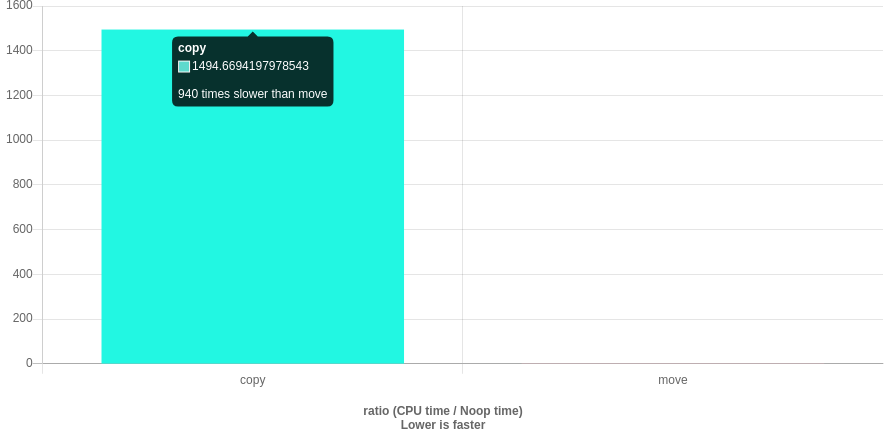
\includegraphics[height=.8\textheight]{benchmark_vec_mv.png}
\end{frame}

\begin{frame}[plain,noframenumbering]
    \centering
    \scalebox{3}{Universal References}
\end{frame}

\section{Universal References}

\begin{frame}[fragile]{Rvalue ref. or no rvalue ref.?}
    Rvalue refs are declared using \enquote{\&\&}: reasonable to assume that the presence of \enquote{\&\&} in a type declaration indicates an rvalue reference?
    \only<2>{\textbf{No!}}
    \begin{columns}
        \begin{column}{.45\textwidth}
            \begin{lstlisting}[numbers=none]
struct S{};

S&& s = S{};                // (1)

auto&& s2 = s;              // (2)

void f(S&& s);              // (3)

template <typename T>
void f(T&& t);              // (4)

template <typename T>
void f(const T&& t);        // (5)

template <typename T>
void f(std::vector<T>&& v); // (6)
            \end{lstlisting}
        \end{column}
        \begin{column}{.5\textwidth}
            \textbf{Does \enquote{\texttt{\&\&}} mean rvalue reference?}
            \begin{itemize}
                \item \texttt{(1)}: \only<1>{???}\only<2>{yes}
                \item \texttt{(2)}: \only<1>{???}\only<2>{no}
                \item \texttt{(3)}: \only<1>{???}\only<2>{yes}
                \item \texttt{(4)}: \only<1>{???}\only<2>{no}
                \item \texttt{(5)}: \only<1>{???}\only<2>{yes}
                \item \texttt{(6)}: \only<1>{???}\only<2>{yes}
            \end{itemize}
        \end{column}
    \end{columns}
\end{frame}

\begin{frame}[fragile]{Universal references}
    \begin{columns}
        \begin{column}{.5\textwidth}
            \textbf{Universal references${}^{\color{vertexDarkRed}\star}$}
            \begin{itemize}
                \item Syntax (\texttt{x} is a universal reference):
                \begin{itemize}
                    \item \texttt{auto\&\& x}
                    \item \texttt{template <typename T>} \texttt{f(T\&\& x\ldots}
                \end{itemize}
                \item Rule of thumb: substitute fully qualified type into \texttt{auto} or \texttt{T} and reduce:
                \begin{itemize}
                    \item \texttt{\&\&} $\mapsto$ \texttt{\&\&} 
                    \item \texttt{\&\&\&} $\mapsto$ \texttt{\&} 
                    \item \texttt{\&\&\&\&} $\mapsto$ \texttt{\&\&} 
                \end{itemize}
            \end{itemize}
        \end{column}
        \begin{column}{.45\textwidth}
            \begin{lstlisting}[numbers=none]
std::vector<S> v;
auto&& s = v[0]; // S&&& -> S&

auto&& s2 = S{}; // S&&&& -> S&&
auto&& s3 = s2;  // S&&&  -> S&

// S&&&& -> S&&
auto&& s3 = std::move(s2);
            \end{lstlisting}
        \end{column}
    \end{columns}

    \vspace{5mm}

    \footnotesize ${}^{\color{vertexDarkRed}\star}$ \textit{Universal reference}: term introduced by Scott Meyers
\end{frame}

\begin{frame}[fragile]{Q: What is the output of the program?}
    \inputcpplisting{snippet35a}
\end{frame}

\begin{frame}[fragile]{A: \texttt{abb}}
    \inputcpplisting{snippet35a}

    \hfill \ldots how to preserve the value category?
\end{frame}

\begin{frame}[fragile]{Q: What is the output of the program?}
    \inputcpplisting{snippet37}
\end{frame}

\begin{frame}[fragile]{A: \texttt{aba}}
    \inputcpplisting{snippet37}
\end{frame}

\begin{frame}[fragile]{Q: What is the output of the program?}
    \inputcpplisting{snippet38}
\end{frame}

\begin{frame}[fragile]{A: \texttt{abaa}}
    \inputcpplisting{snippet38}
\end{frame}

\begin{frame}[fragile]{Perfect forwarding}
    \centering
    \scalebox{1.5}{How do we fuse these implementations?}

    \begin{lstlisting}
// if `t` is an lvalue of type `S`
S& forward(S& t) {
    return t;
}

// if `t` is an rvalue of type `S`
S&& forward(S& t) { // not `S&&`!
    return std::move(t); // static_cast<S&&>(t)
}
    \end{lstlisting}

    \inputcpplisting{snippet36}
\end{frame}

\begin{frame}[fragile]{Q: What is the output of the program?}
    \inputcpplisting{snippet35b}
\end{frame}

\begin{frame}[fragile]{A: \texttt{abc}}
    \inputcpplisting{snippet35b}
    \textbf{Rule of thumb:} Use \texttt{std::move} for rvalues and \texttt{std::forward} for universal references
\end{frame}

\begin{frame}[fragile]{Q: Why can't we use perfect forwarding here?}
    \inputcpplisting{snippet9}

    \only<2>{\textbf{A:} The first call in the loop might \textit{steal} the values, leading to unexpected behavior calling \texttt{op} in subsequent iterations.}
\end{frame}

\begin{frame}[plain,noframenumbering]
    \centering
    \scalebox{3}{Reading x86-64 Assembly}

    \scalebox{2}{\ldots for fun and profit}
\end{frame}

\section{Reading Assembly for Fun and Profit}

\begin{frame}[fragile]{Function Prologue \& Epilogue}
    \begin{itemize}
        \item Few lines of code at the beginning (\textit{prologue}) and end (\textit{epilogue}) of a function, which \textbf{prepare}
        \begin{itemize}
            \item the \textbf{stack} and 
            \item \textbf{registers}
        \end{itemize}
        \item Not part of assembly: \textbf{convention} (defined \& interpreted differently by different OS and compilers)
    \end{itemize}

    \begin{columns}[t]
        \begin{column}{.45\textwidth}
            \textbf{Prologue}
            \begin{lstlisting}[language={}]
push rbp
mov rbp, rsp
sub rsp, N
            \end{lstlisting}
            alternatively
            \begin{lstlisting}[language={}]
enter N, 0
            \end{lstlisting}
            (reserve \texttt{N} bytes on stack for local use)
        \end{column}
        \begin{column}{.45\textwidth}
            \textbf{Epilogue}
            \begin{lstlisting}[language={}]
mov rsp, rbp
pop rbp
ret
            \end{lstlisting}
            alternatively
            \begin{lstlisting}[language={}]
leave
ret
            \end{lstlisting}
        \end{column}
    \end{columns}
\end{frame}

\begin{frame}[fragile]{Stack frame for function call}
    \begin{columns}
        \begin{column}{.4\textwidth}
            \begin{itemize}
                \item \texttt{CALL} = \texttt{PUSH} \textit{address of next instruction} + \texttt{JMP} \textit{target}
                \item \texttt{RET} pops return address and transfers control there
                \item pass arguments 1 \ldots 6 in registers (\texttt{rsi}, \texttt{rdx}, \ldots)
            \end{itemize}
        \end{column}
        \begin{column}{.6\textwidth}
            \begin{Verbatim}
┌──────────────┐
│ ...          │
│ 8th Argument │ (rbp + 24)
│ 7th Argument │ (rbp + 16)
├──────────────┤
│ rip          │ (return address)
│ rbp          │ (rbp)
├──────────────┤
│ rbx          │
│ r12          │
│ r13          │ (rsp)
└──────────────┘
            \end{Verbatim}
            (stack frame for function call with 8 arguments and local registers \texttt{rbx}, \texttt{r12} and \texttt{r13})
        \end{column}
    \end{columns}
\end{frame}

\begin{frame}[fragile]{\texttt{lea} vs. \texttt{mov}}
    \begin{columns}
        \begin{column}{.5\textwidth}
            \begin{itemize}
                \item \texttt{lea}: \underline{l}oad \underline{e}ffective \underline{a}ddress
                \item puts memory address from \texttt{src} into the destination \texttt{dest}
                \item Example: \texttt{lea eax, [ebx+8]}
                \begin{itemize}
                    \item put \texttt{[ebx+8]} into \texttt{eax}
                    \item value of \texttt{eax} after instruction: \texttt{0x00403A48}
                \end{itemize}
                \item \ldots whereas: \texttt{mov eax, [ebx+8]}
                \begin{itemize}
                    \item value of \texttt{eax} after instruction: \texttt{0x0012C140}
                \end{itemize}
            \end{itemize}
        \end{column}
        \begin{column}{.5\textwidth}
            \begin{Verbatim}
           ┌──────────────────┐
           │ Registers        │
           ├──────────────────┤
           │ EAX = 0x00000000 │ 
           │ EBX = 0x00403A40 │ 
           └──────────────────┘
           ┌────────────┐
           │ Memory     │
           ├────────────┤
0x00403A40 │ 0x7C81776F │ 
0x00403A44 │ 0x7C911000 │ 
0x00403A48 │ 0x0012C140 │ 
0x00403A4C │ 0x7FFDB000 │ 
           └────────────┘
            \end{Verbatim}
        \end{column}
    \end{columns}
\end{frame}

\begin{frame}[fragile]{Reading assembly for fun and profit}
    \begin{columns}[t]
        \begin{column}{.45\textwidth}
            \inputcpplisting{snippet5a}
            
            \only<2>{%
            \inputasmlisting{snippet5b}}
        \end{column}
        \begin{column}{.45\textwidth}
            \inputasmlisting{snippet5a}
        \end{column}
    \end{columns}
\end{frame}

\begin{frame}[fragile]{Reading assembly for fun and profit}
    \begin{columns}[t]
        \begin{column}{.45\textwidth}
            \inputcpplisting{snippet6a}

            \only<2>{%
            \inputasmlisting{snippet6b}}
        \end{column}
        \begin{column}{.45\textwidth}
            \inputasmlisting{snippet6a}
        \end{column}
    \end{columns}

\end{frame}

\begin{frame}[fragile]{Reading assembly for fun and profit}
    \begin{columns}[t]
        \begin{column}{.45\textwidth}
            \inputcpplisting{snippet1a}
        \end{column}
        \begin{column}{.45\textwidth}
            \inputasmlisting{snippet1a}
        \end{column}
    \end{columns}
\end{frame}


\section{Implicit Costs of \texttt{const\&}}

\begin{frame}[fragile]{Implicit Costs of using \texttt{const\&}}
    \begin{columns}[t]
        \begin{column}{.45\textwidth}
            \inputcpplisting{snippet1a}
        \end{column}
        \begin{column}{.45\textwidth}
            \inputcpplisting{snippet2a}
        \end{column}
    \end{columns}
\end{frame}

\begin{frame}[fragile]{Implicit Costs of using \texttt{const\&}}
    \begin{columns}[t]
        \begin{column}{.45\textwidth}
            \inputasmlisting{snippet1a}
        \end{column}
        \begin{column}{.45\textwidth}
            \inputasmlisting{snippet2a}
        \end{column}
    \end{columns}
\end{frame}

\begin{frame}[fragile]{Implicit Costs of using \texttt{const\&}}
    \begin{columns}[t]
        \begin{column}{.45\textwidth}
            \inputasmlisting{snippet1b}

            \footnotesize
            \only<2>{\textbf{NB \#1:} adjusting \texttt{rsp} in function prologue necessary when function is not a leaf function since callee have to know where to start saving variables on stack. (Adjusting \texttt{rsp} can be ommitted in leaf functions.)}
            \only<3>{\textbf{NB \#2:} Offset \texttt{x} in \texttt{sub rsp, x} is objective of optimizations such as alignment: ABI requires stack to be aligned to 16 bytes.}
        \end{column}
        \begin{column}{.45\textwidth}
            \inputasmlisting{snippet2b}
        \end{column}
    \end{columns}
\end{frame}

\begin{frame}[fragile]{Will it compile?}
    \begin{columns}
        \begin{column}{.45\textwidth}
            \inputcpplisting{snippet39}
        \end{column}
        \begin{column}{.45\textwidth}
            \only<2>{%
            \textbf{\textcolor{vertexDarkRed}{No!}}
            \begin{itemize}
                \item Constructor takes by reference
                \item References to automatic storage objects are not constant expressions!
                \item Solutions?
            \end{itemize}}
        \end{column}
    \end{columns}

    \vspace{1cm}

    \begin{lstlisting}
template <std::size_t N>
constexpr span(const std::array<value_type, N>& arr) noexcept;
    \end{lstlisting}
    \href{https://en.cppreference.com/w/cpp/container/span/span}{\texttt{cppreference.com/w/cpp/container/span/span}}
\end{frame}

\begin{frame}[fragile]{Will it compile?}
    \inputcpplisting{snippet40}
\end{frame}

\begin{frame}[fragile]{Nota bene \ldots}
    this will work though, since reference / pointer does not \textit{escape} constant expression \ldots
    \inputcpplisting{snippet41}
\end{frame}
